\documentclass{amsart}
\usepackage{amssymb, amsmath, graphicx, caption, enumerate}
\graphicspath{ {images/} }
\usepackage{amsthm}
\usepackage{xargs}
\usepackage{scalerel}
\usepackage[ ]{algorithm2e}
\usepackage[dvipsnames]{xcolor}

\makeatletter
\renewcommand{\@algocf@capt@plain}{above}% formerly {bottom}
\makeatother


\newcommand{\D}{\mathcal{D}}
\newcommand{\A}{\mathcal{A}}
\newcommand{\N}{\mathbb{N}}
\newcommand{\Z}{\mathbb{Z}}
\newcommand{\R}{\mathbb{R}}
\newcommand{\K}{\mathbb{K}}
\newcommand{\C}{\mathbb{C}}
\newcommand{\mustar}{\mu^*}
\newcommand{\ds}{\displaystyle}
\newcommand{\op}[1]{\left(#1\right)}
\newcommand{\cp}[1]{\left[#1\right]}
\newcommand{\av}[1]{\left| #1\right|}
\newcommand{\st}[1]{\left\{#1\right\}}




\usepackage[colorinlistoftodos,prependcaption,textsize=tiny]{todonotes}
\newcommandx{\question}[2][1=]{\todo[linecolor=red,backgroundcolor=red!25,bordercolor=red,#1]{#2}}
\newcommandx{\change}[2][1=]{\todo[linecolor=blue,backgroundcolor=blue!25,bordercolor=blue,#1]{#2}}
\newcommandx{\add}[2][1=]{\todo[linecolor=OliveGreen,backgroundcolor=OliveGreen!25,bordercolor=OliveGreen,#1]{#2}}
\newcommandx{\improve}[2][1=]{\todo[linecolor=Plum,backgroundcolor=Plum!25,bordercolor=Plum,#1]{#2}}
\newcommandx{\thiswillnotshow}[2][1=]{\todo[disable,#1]{#2}}
\newcommandx{\remove}[2][1=]{\todo[linecolor=yelllow,backgroundcolor=yellow!10,bordercolor=red,#1]{#2}}


\newcommand\reallywidehat[1]{\arraycolsep=0pt\relax%
\begin{array}{c}
\stretchto{
  \scaleto{
    \scalerel*[\widthof{\ensuremath{#1}}]{\kern-.5pt\bigwedge\kern-.5pt}
    {\rule[-\textheight/2]{1ex}{\textheight}} %WIDTH-LIMITED BIG WEDGE
  }{\textheight} % 
}{0.5ex}\\           % THIS SQUEEZES THE WEDGE TO 0.5ex HEIGHT
#1\\                 % THIS STACKS THE WEDGE ATOP THE ARGUMENT
\rule{-1ex}{0ex}
\end{array}
}

\setlength{\textwidth}{\paperwidth}
\addtolength{\textwidth}{-3in}
\calclayout

%\setcounter{secnumdepth}{0}
%\usepackage{titlesec}
%\titleformat{\section}{\Large\bfseries}
%\titleformat{\subsection}{}






\begin{document}





\begin{abstract}

  
We consider maps $f$ with additive or multiplicative noise from a high-dimensional parameter space $\Lambda$ to a data space $\mathcal{D}$ of lower dimension, where $\nabla f$ exists, but may be inaccessible. Many problems in Uncertainty Quantification require minimizing such an $f$. We investigate Derivative-Free Optimization (DFO) in this setting. The considered DFO algorithm's hyperparameters depend on two generally unknown parameters -- the $L_1$ Lipschitz constant of $f$ and the bounded variance in the noise of $f$, $\sigma^2$. We firstly explore efficiently learning $L_1$ and $\sigma^2$ from samples. To learn $L_1$, approximations to $\nabla^2 f$ are needed. 
Secondly, we examine methods of enhancing the DFO algorithm by performing dimension reduction in $\Lambda$.  
The DFO hyperparmeters are inversely proportional to the known dimension $P$ of $\Lambda$, resulting in heavy smoothing and small step sizes for large $P$.
By learning a lower-dimensional \textit{active subspace} $\mathcal{A}$ of $f$ which defines directions causing the majority of the variance of $f$, iterates in a DFO algorithm may be updated with steps only taken in $\mathcal{A}$, reducing the value of $f$ more efficiently than updating iterates in the full variables, $\Lambda$. 
Dimension reduction can be performed with access to samples  and does require approximations to $\nabla f$. In addition to computational savings made by stepping only in active directions when an active subspace exists, computational costs may be reduced further by learning hyperparameters and the active subspace from DFO iterates whenever possible, reducing map evaluations.

 

\end{abstract}


\title{Optimizing Noisy, High-Dimensional Functions}

\author{Jordan R. Hall}

\maketitle


% TOC
\setcounter{tocdepth}{1} 
\tableofcontents






\newpage


\section{Introduction}


We begin our discussion by defining a parameter space $\Lambda$ of dimension $P$,  a data space $\mathcal{D}$, and a  map or ``model" $f: \Lambda \rightarrow \mathcal{D}$.
%, such that $f(\lambda) \subseteq \mathcal{D}:=f(\Lambda)$. 
We assume that $\mathcal{D}$ has dimension $D$, typically with $D<< P$. Most of the discussion will focus on the case $\mathcal{D} \subseteq \mathbb{R}$. 
Points in $\mathcal{D}$ may be known values of $f(\lambda), \lambda\in \Lambda$; as such, we may write $d=f(\lambda)$ to denote the particular datum corresponding to the evaluation of a point $\lambda \in \Lambda$ under $f$. 
Points in $\mathcal{D}$ may also be \textit{observed} data, denoted $d_{\text{obs}}$, where the corresponding $\lambda\in \Lambda$ may be unknown. 
We assume realizations of $f$ are  noisy. We model such observations of $f$ with $d_{\text{obs}}=\hat{f}(\lambda;\xi)=f(\lambda)+\epsilon(\xi)$(additive noise)  or $d_{\text{obs}}=\hat{f}(\lambda;\xi)=f(\lambda)(1+\epsilon(\xi))$(multiplicative noise). In both cases $\epsilon(\cdot)$ denotes a random variable specified by realizations or draws $\epsilon(\xi)$. We assume $\epsilon(\cdot)$ has bounded variance $\sigma^2<\infty$.


Many objective functions formed in Uncertainty Quantification (UQ) applications generally fall into the category of maps $f$ described above. For example, one may solve a \textit{Stochastic Inverse Problem} (\textit{SIP}) by posing an equivalent deterministic optimization problem, with the heavy assumptions that $f$ is a linear map and the \textit{prior distribution} in $\Lambda$ and \textit{observed distribution} in $\mathcal{D}$ are Gaussian. Optimizing $f$ in the setting described above is an example  of \textit{Optimization Under Uncertainty} (\textit{OUU}).

In this section we provide a brief literature review and discussion of Derivative-Free Optimization (DFO), hyperparameter learning, and dimension reduction. We introduce a theoretical framework to unify results in the literature so that we may propose methods and state results in the proceeding sections.




\subsection{Derivative-Free Optimization}

Many important physical systems possess turbulent or chaotic behavior.  The physical state of the system $u(x,\lambda)$ and the corresponding parameter
to observable map $f(u(x,\lambda))$ may be modeled as a stochastic process, or as a deterministic function with additive or multiplicative noise.  
In this setting, the efficient extraction of accurate gradients of $f$ in parameter space is a challenging undertaking, as popular techniques based on
linearization, including adjoint methods, are inaccurate \cite{lea2000, Qiqi2014}.  
The finite-difference approximations to $\nabla f_\Lambda$ 
involve  $P=\text{dim}(\Lambda)$ 
additional, usually nonlinear model solves for the physical system state $u(x,\lambda_i + \delta \lambda_i)$, and are greatly polluted by the noise in $f$.

As a consequence of these difficulties, optimization in this setting will need to be performed by algorithms which
do not require  gradient approximation. % from samples while online; 
Otherwise, we expect to surpass a reasonable computational budget since as even one gradient approximation will involve $\mathcal{O}(P)$  evaluations of $f$(using, for instance, finite differencing).
We consider \textit{Derivative-Free Optimization} (DFO) algorithms suited for additive and multiplicative noise. DFO algorithms require nothing more than the ability to evaluate the noisy model $f$ and randomly draw from a normal distribution; $\nabla f$ is not required. %unneeded once inputs and algorithm hyperparameters have been prescribed.

Given an initial guess $\lambda^{(0)}$, many DFO algorithms find subsequent iterates $\lambda^{(k)}$ by random walks or \textit{ball walks} in $\Lambda$ specified by draws from a $P$-dimensional Gaussian distribution.
% in every coordinate of $\lambda^{(k)}$; 
Iterates are controlled by prescribed hyperparameters, such as smoothing factors and step sizes. 
%Hyperparameters (e.g. smoothing factor and step size) in DFO algorithms are of great importance to their convergence. 
These hyperparameters often depend on potentially unknown properties of the model $f$.
For example, in the STARS algorithm\cite{CW}, the hyperparameters depend on the variance of the noise $\epsilon(\xi)$ and the $L_1$ Lipschitz constant of $f$.  We discuss strategies for learning model properties to tune DFO hyperparameters in Section \ref{ss:hyper_learn}.
%Both the smoothing factor and step size depend on the $L_1$ Lipschitz constant of $f$. As such, it %will be of interest to obtain estimates of $L_1$, which is not straightforward in a gradient-free setting. We refer to \cite{Calliess} for Lipschitz constant learning in this setting, and discuss this problem more in the proceeding subsection.

As in \cite{CW}, we consider the additive noise OUU problem

\begin{eqnarray} \label{eq:1}
\min_{\lambda \in \Lambda} \quad \mathbb{E}\left[f(\lambda)+\epsilon(\xi)\right],
\end{eqnarray} 

\noindent and the multiplicative noise OUU problem

\begin{eqnarray} \label{eq:2}
\min_{\lambda \in \Lambda} \quad \mathbb{E}\left[f(\lambda)(1+\epsilon(\xi))\right],
\end{eqnarray} 

\noindent where the authors assume:

\begin{enumerate}[(i.)]

\item $f: \Lambda=\R^P \to \R-\D$ is continuously differtiable, convex, and $\nabla f$ has Lipschitz constant $L_1$

\item $\epsilon(\cdot)$ is a random variable with probability density $\pi_{\epsilon}(\epsilon(\xi))$;

\item for all $\lambda$ the noise $\epsilon(\cdot)$ is independent and identically distributed, has bounded variance $\sigma^2$, and is unbiased; i.e., $\mathbb{E}_\xi (\epsilon(\xi))=0$;

\item for multiplicative OUU, the additional assumptions that: the \textit{signal-to-noise ratio} is bounded -- i.e., $\mathbb{E}((1+\epsilon(\xi))^{-1})<b$ -- and the support of $\epsilon(\xi)$ is bounded by $\pm a$, $a<1.$

\end{enumerate}




In \cite{CW} the \textit{STARS (STep-size Approximation in Randomized Search)} DFO algorithm is used to solve the additive and multiplicative OUU problems \eqref{eq:1},\eqref{eq:2} under the  assumptions (i.)-(iv.). Briefly, STARS uses small perturbations of iterates in $\Lambda$ by the addition of a random vector with components drawn from a normal distribution, computes the noisy function value at the randomly perturbed point, and updates iterates using a Gaussian-smoothed finite-difference for approximate gradient information in a gradient-descent-type scheme. STARS only  requires the ability to evaluate $f$ and access to random draws from a normal distribution. All in all, the algorithm can be implemented in about 10 lines of code in any standard computing language; we used Python 3 for the STARS results presented in this paper. 

As mentioned above, STARS has two primary hyperparameters, the smoothing factor $\mu^*$ and the stepsize $h$.
%Both the smoothing factor and step size depend on the $L_1$ Lipschitz constant of $f$. As such, it will be of interest to obtain estimates of $L_1$, which is not straightforward in a gradient-free setting. We refer to \cite{Calliess} for Lipschitz constant learning in this setting, and discuss this problem more in the proceeding subsection.
We witness best performance in STARS when these two hyperparameters are %the algorithm 
near their optimal values. We now discuss learning these important hyperparameters algorithmically.


\subsection{Learning Hyperparameters}  \label{ss:hyper_learn}
STARS, like many DFO algorithms, exhibits optimal convergence if and only if its hyperparameters -- namely the smoothing factor and step size -- are properly tuned. The smoothing factor and step size for STARS will be precisely defined in  Section \ref{ss:methods_stars}; for now, it is enough to state that these hyperparameters depend on the bounded variance in the noise $\sigma^2$,  the $L_1$ Lipschitz constant of the objective function $f$, and 
\footnote{i.e., the value $L_1> 0: ||\nabla f(\lambda^1)-\nabla f(\lambda^2)|| \leq L_1 ||\lambda^1 -\lambda^2||$ $\forall \lambda^1, \lambda^2 \in \Lambda$, where $||\cdot||$ denotes a norm on $\Lambda$ (which is a \textit{normed linear space}).}
%which are both generally unknown,
the known $\dim \Lambda=P$. %which is assumed to be known. 

Tuning the hyperparameters in STARS is a matter of learning $\sigma^2$ and $L_1$. In this paper, we propose algorithmic methods of learning STARS hyperparameters so that one need not specify the hyperparameters at all, fully automating the process of solving optimization problems \eqref{eq:1} and \eqref{eq:2}. 
%Since we are considering $f$ to be a a black-box, it is unrealistic to assume that a user would know $\sigma^2$, much less $L_1$, which would require at least some type of gradient information.

To learn the variance in the noise, we rely on the ECNoise algorithm \cite{MW} which even for $P$ large requires few evaluations of $f$ -- often 6 to 10 evaluations will suffice. Briefly, ECNoise uses a series of nearby samples $s^i:=(\lambda^i,f(\lambda^i))$ of points $\lambda^i$ along a line in $\Lambda$. Forming a classical difference table of iterative residuals, the authors show that estimators $\hat{\sigma^2}$ to $\sigma^2$ are formed. Learning $\sigma^2$ is performed prior to STARS, and may be viewed as a computational expense we must pay up front to ensure convergence of the algorithm.

Learning $L_1$ in this setting is more of a challenge, mainly to our postulated %since we assume that we 
lack of access to $\nabla f$. Given $S$ pointwise estimates to the gradient, which we denote with $\hat{\nabla}f(\lambda^i)$, $i=1,\ldots, S$, we could consider an estimator such as



\begin{equation} \label{eq:3}
\reallywidehat{L_1}:= \max_{i \neq j} \frac{\left|\left|\reallywidehat{\nabla f}(\lambda^{i})-\reallywidehat{\nabla f}(\lambda^{j})\right|\right|-2\epsilon^*}{||\lambda^{i}-\lambda^{j}||}, \quad \epsilon^*=\sup_\xi |\epsilon(\xi)|, \quad i,j=1,\ldots, S,
\end{equation} 

\noindent which is %a ``bad idea" 
given in \cite{Calliess}. There are several problems with such an approach. Mainly, forming $\hat{\nabla} f$ is expensive, requiring at least $P+1$ evaluations of $f$ for each approximation. Even if one uses only 3 samples $s_i$, $i=1,2,3$, forming $\hat{L_1}$ requires $3(P+1)$ $f$ evaluations, which will often exceed the number of function evaluations needed for STARS to converge, assuming its hyperparameters are reasonably tuned.

Another challenge involves specifying $\epsilon^*$ in \eqref{eq:3}, which is subtracted from the estimator's numerator to control for noise in $f$. To save computational expense, we propose forming an initial estimate to $L_1$ by recycling function values from ECNoise in a finite-difference fashion. Then, once STARS is initiated, $L_1$ can be updated using information from approximate directional derivatives formed from iterates (and their corresponding function values). In fact, the iterates (and intermediate iterates) formed during STARS lend themselves naturally for finite differencing to estimate $L_1$.

%Both hyperparmeters must be adjusted if dimension reduction is performed because both values depend on $P$. We note that both parameters in fact have an inverse proportionality with $P$. Hence, if $\Lambda$ permits dimension reduction to $k$ \textit{active directions} where, say, $k<<P$, both hyperparemeters will be larger using $k$ for $\dim \Lambda$ instead of $P.$ We now turn to introducing dimension reduction in our setting.





\subsection{Dimension Reduction}
We consider functions from a high-dimensional space $\Lambda$ to a data space $\D$ of smaller dimension; i.e., $\dim \D << \dim \Lambda$. Many functions of interest
actually represent postprocessed quantities from the solution of complex physical models. 
It is not often the case that every parameter has an equal impact on function values; usually some parameters matter more than others. If it is possible to mimic the response of $f$ by processing fewer parameters, we can expect computational savings.

We consider Active Subspace (AS) methods described by Paul Constantine in \cite{Constantine2015} and an equivalent method by T.M. Russi in \cite{Russi}. These techniques seek to explain outputs $f(\Lambda)$ in a subspace $\A \subset \Lambda$ for which the $\dim (\A) <P$ or perhaps $\dim(\A)<<P$. Here we discuss the theoretical formulation of $\A$. The details of finding $\A$ algorithmically is discussed in the proceeding section.

We note that AS requires, at the very least, approximations to $\nabla f$. For the discussion in this section, we continue with the understanding that $\nabla f$ is approximatied in some fashion, the details of which will be discussed in the proceeding Methods section. We assume that $\nabla f(\lambda)$ %s $P\times 1$ containing the $P$ partial derivatives of $f$, which for this discussion we assume exist,
 is square integrable in $\Lambda$ with respect to %a equipped with some
 probability density $\pi_\Lambda(\lambda)$ that is positive everywhere in $\Lambda$ and 0 otherwise.
 
In AS(and many other dimension reduction techniques\cite{Russi}), we transform inputs $\lambda$ to a bounded domain %the origin 
with some fixed variance, typically so that $\lambda\in [-1,1]^P$. Then, as in \cite{ConstantineMC}, we write the \textit{sensitivity matrix}

\begin{equation} \label{eq:4}
W=\int_\Lambda \nabla f(\lambda) \nabla f(\lambda)^\top  \pi_\Lambda(\lambda) d\lambda,
\end{equation} 

\noindent which is a $P\times P$ symmetric positive semi-definite matrix defining a certain covariance of $\nabla f$ in $\Lambda$. This interpretation of \eqref{eq:4} suggests the computation of the eigendecomposition of $W$ %leads one to the idea of computing the Singular Value Decomposition (SVD) of $W$,

\begin{equation} \label{eq:5}
W=VDV^*,
\end{equation} 

\noindent where $V$ is $P \times P$ unitary with columns given by the eigenvectors $v_i$ of $W$ and $D$ is a diagonal matrix containing the ordered eigenvalues of $W$, $\{d_i\}$. % $\Sigma$ is $P \times P$ diagonal with the singular values of $W$ along its diagonal, and $V^*$ is $P \times P$ unitary.
%With the singular values of $W$ in hand from its SVD, 
To find the active subspace, %we search for a drop-off in the spectrum of $W$. 
we seek %one may plot the singular values, $\{\sigma_i\}_{i=1}^P$ and seek 
a drop-off in magnitude between some pair of eigenvalues, $d_{j}$ and $d_{j+1}$, $1\leq j \leq j+1 \leq P$, where $d_{j}>>d_{j+1}$. The active subspace of $f$ is the span of $v^1,\ldots,v^{j}$, which we denote % which are the first $j$ columns of $V$. %, the right singular vectors of $W$. We let
\begin{equation} \label{eq:6}
\A(f)=\text{span}\{v^1,\ldots,v^j\}.
\end{equation}

%\noindent denote the \textit{active subspace} of $f$.


The fact that $v^1,\ldots,v^{j}$ correspond to large %the nontrivial singular values 
eigenvalues is exactly why they account for the most amount of variance in function values. In fact, one can view AS as an artful choice of principal components after a \textit{full} Principal Component Analysis (PCA) is performed in the gradient space $W$; for more details on this viewpoint, we refer the reader to Section 6.4 in \cite{Russi}.

For a point $\lambda \in \Lambda$, we define

\begin{equation} \label{eq:7}
  \mathcal{P}_\A(\lambda)=\sum_{i=1}^{j}\left( ({v^i})^T \lambda\right)v^i \in \A, 
\end{equation}

\noindent which is a projection of the point $\lambda$ in the active subspace of $f$. We call this projection an \textit{active variable}, which is a point in the active subspace $\A$. We have arrived at the property that 

\begin{equation} \label{eq:8}
f\left(\mathcal{P}_\A(\lambda)\right) \approx f(\lambda).
\end{equation}

The above property  gives the ability to save computational expense in many scenarios in UQ, 
%for a number of problems in Uncertainty Quantification, 
including optimization, approximation %representation 
and solving inverse problems. 

%\vspace{1cm}

With the literature review and introduced notation provided above, the remaining sections focus on methodology, results, and conclusions. 

In the proceeding Methods section (\ref{s:Methods}, we % thoroughly 
discuss the details of the STARS algorithm, algorithmic hyperparameter learning, and Monte Carlo-style AS, which are the key ingredients needed to perform STARS performed only in the active directions. We then discuss the techniques used to create the fully-automoted \textit{Active STARS} algorithm.

In the Results section (\ref{s:Results}), we consider 2 model problems %with maps that mimic the behavior of the noisy "black box''  we consider. 
We compare learned hyperparameters to their true values, which are specified by the example functions we choose. We also compare the performance of STARS in full variables to automated Active STARS.

Finally, in the Conclusion and Discussion section (\ref{s:Conc}), we review the extent to which active STARS is effective in our setting. Limitations are discussed and future research questions are posed. 

\section{Methods}  \label{s:Methods}

In the following, we begin by detailing STARS, learning its hyperparameters, and learning the active subspace of $f$. Then, we propose a modification to STARS so that steps are taken in active directions only. Finally, we combine ingredients, proposing a fully automated Active STARS where hyperparameters and the active subspace are learned online, using information from iterates.


\subsection{STARS}  \label{ss:methods_stars}

We first present STARS suited for additive or multiplicative OUU as in \eqref{eq:1} and \eqref{eq:2} in the  pseudocode below.

\vspace{.25cm}


\begin{algorithm}[H]

\SetAlgoLined

	\KwIn{\texttt{maxit}$=:M$; $\lambda^{(0)}$; $f_0:=f(\lambda^{(0)})$; $h$; $k=1$}
 
    \While{$k\leq M$}{
    
  Form smoothing factor $\mu^*_k$
    
  Draw $u^{(k)}$, where $u^{(k)}_p \sim N(0,1)$ for $p=1,\ldots,P$\;
  
  Evaluate $g_k:=f(\lambda^{(k-1)}+\mu^*_ku^{(k)})$\;
  
  Set $ d^{(k)}:=\frac{g_k-f_{k-1}}{\mu^*_k}u^{(k)}$\;
  
  Set $\lambda^{(k)}=\lambda^{(k-1)}-h\cdot d^{(k)}$\;
  
  Evaluate $f_k:=f(\lambda^{(k)})$\; 
  
  Set $k=k+1$\;}

    \KwOut{($\lambda^{(M)}$, $f_M$)}

	\caption{STARS for Additive or Multiplicative OUU}

\end{algorithm}

\vspace{.25cm}

\noindent Observe that STARS requires defining hyperparameters $\mu^*_k$ and $h$, which are the algorithm's smoothing factor and step size, respectively. The step length $h$ will remain constant for all iterations regardless; in the case of of  Multiplicative OUU, 
%In the case of Additive OUU, $\mu^*_k$ will also be constant, i.e., $\mu^*_k=\mu^*$, a fixed value for all iterations $k=1, \ldots, M$. However in the case of Multiplicative OUU, 
the smoothing factor $\mu^*_k$ will need to be adjusted at every iteration $k$.  

For the additive noise OUU problem \eqref{eq:1}, the values for $\mu^*$ and $h$ are 

\begin{eqnarray} \label{eq:9}
\mu^*:=\left( \frac{8\sigma^2 P}{L_1^2(P+6)^3}\right)^{1/4} \quad \quad h:=(4L_1(P+4))^{-1},
\end{eqnarray} 

\noindent which are proven as optimal values for the algorithm's convergence in \cite{CW}. 

Assume $f$ and its additive noise $\epsilon(\cdot)$ obey assumptions (i.)-(iii.), and let $f_*:=f(\lambda^*)$ where $\lambda^*$ denotes the true minimizer of $f$ and $f_k:=f(\lambda^{(k)})$ where $\{\lambda^{(k)}\}$ denotes a sequence of iterates formed from STARS (Algorithm 1). Then for any maximum iteration count $M \geq 0$,

\begin{eqnarray} \label{eq:10}
\frac{1}{M+1} \sum_{k=0}^M (f_k-f_*) \leq \frac{4L_1(P+4)}{M+1}||\lambda^{(0)}-\lambda^*||^2 + \frac{3 \sqrt{2}}{5} \sigma (P+4),
\end{eqnarray} 

\noindent where $||\cdot||$ denotes the Euclidean norm in $\Lambda= \R^P$.

In the multiplicative noise OUU problem \eqref{eq:2}, the step length $h$ remains the same, exactly as in \eqref{eq:9} above, held constant for each iteration. However the smoothing factor must be updated for each iteration $k=1,\ldots, M.$ As shown in \cite{CW}, the optimal smoothing factor for a given iterate $k$ is given by

\begin{eqnarray} \label{eq:11}
\mu^*_k:=\left( \frac{16 \sigma^2 f(\lambda^{(k)};\xi_k)^2 P}{L_1^2(1+3\sigma^2)(P+6)^3}\right)^{1/4}.
\end{eqnarray} 

Assume $f$ and its additive noise $\epsilon(\cdot)$ obey assumptions (i.)-(iv.), and let $\{\lambda^{(k)}\}$ denote a sequence of iterates formed from STARS (Algorithm 1). Then for any maximum iteration count $M \geq 0$,

\begin{eqnarray} \label{eq:12}
\frac{1}{M+1} \sum_{k=0}^M (f_k-f_*) \leq \frac{4L_1(P+4)}{M+1}||\lambda^{(0)}-\lambda^*||^2 + 4L_1(P+4)(K_1B +K_2),
\end{eqnarray} 


\noindent where $B$ denotes an upper bound for the average of the absolute value of function evaluations $|f(\lambda^{(k)})|$, $k=1,\ldots,M$, and $K_1$ and $K_2$ are long-form constants; the interested reader may refer to \cite{CW}.

STARS typically converges to a minimum when the hyperparameters $\mu_k^*$ and $h$ are within an order of magnitude of their true values. The closer the user-defined $\mu^*$ and $h$ values are to the truth, the faster STARS converges. If $\mu^*$ and $h$ are underestimated, STARS will take very small and heavily smoothed steps, converging slowly; however, if the values are overestimated, the algorithm may cause divergence, in the sense that function evaluations will grow with each iterate.

It is then of high interest to tune the values $\mu$ and $h$ so that function evaluations are not wasted. In the proceeding subsection, we discuss learning the values $\mu$ and $h$ depend on -- namely $\sigma^2$ and $L_1$.


\subsection{Hyperparameter Learning}

Here we present the methods used for learning $\hat{\sigma}^2$, which denotes the estimated bounded variance in the noise of $f$, and $\hat{L_1}$, which is the gradient-Lipschitz constant of $f$. To learn the noise in $f$, we use ECNoise as in \cite{MW}, which will typically learn $\sigma^2$ within an order of magnitude using only 6-10 evaluations of $f$. In this paper, we use ECNoise prior to STARS or Active STARS. The evaluations of $f$ created by ECNoise allows one to form an estimate $L_1$ in a variety of ways, including via finite differencing, or via the expensive estimator in \eqref{eq:3}. The value of $L_1$ can be updated using iterations and the intermediate function evaluations in STARS using finite differencing and/or gradient information provided by peforming AS.

We first discuss ECNoise. The following definitions provide one with classical $k$-level differences in $f$ with chosen discretization $h_1>0$ where

\begin{equation} \label{eq:13}
\Delta^{h_1,0} f :=f \quad \quad \Delta^{h_1,k+1} f:=\Delta^{h_1,k} f(\lambda+h_1)- \Delta^{h_1,k} f(\lambda), \quad 1>>h_1>0, \quad k \geq 0.
\end{equation}  

\noindent Let $S$ denote the maximum level of differences taken -- i.e., $k=1\ldots S$. Then ECNoise will draw $S$ samples $\lambda^1,\ldots,\lambda^S \in \Lambda$ where only a \textit{base point} $\lambda^1$ is specified, then $\lambda^{i+1}=\lambda^{i}+h_1$, $i=1,\ldots,S$. Then, the $k$-level differences are formed. For a given level $k< S$ we obtain $S-k$ differences. With sufficiently small $h_1$ and only a moderate choice of $k$ (usually $k=2,3,4$ sufficies), the differencing scheme in \eqref{eq:11} leaves one with residuals which estimate $\sigma$ up to a constant $C$ which is explicitly defined in \cite{MW}. The authors define the



\begin{equation} \label{eq:14}
\textit{$k$-th level estimate to $\sigma^2,$}\quad \hat{\sigma_k}^2:=C\sum_{i=1}^{S-k}\left(\Delta^{h_1,k}f(\lambda_i)\right)^2.
\end{equation}  

The authors offer heuristics -- requiring further evalutions of $f$ -- to find the best estimation level $k$. Instead, in this paper, we define an estimator $\hat{\sigma}^2$ by averaging the values $\hat{\sigma_k}^2$ in \eqref{eq:12} above for $k=2,\ldots,S-1.$ Choosing $S\geq 3$ we define,

\begin{equation} \label{eq:15}
 \hat{\sigma}^2:=\sum_{i=2}^{S-1}\frac{\hat{\sigma_i}}{S-2}.
\end{equation}  

The estimator $\hat{\sigma}^2$ in \eqref{eq:13} will typically be close enough to $\sigma^2$ for STARS or Active STARS to converge. As such, we sacrifice searching for the best $\hat{\sigma_k}^2$ to save function evaluations that the heuristic-based methods require, using averaged information from the level $k$ estimators we have already formed.

Given a direction $v \in \Lambda$, ECNoise provides samples of form $s_i=(\lambda^i, f(\lambda^i))$, $i=1,\ldots, S$, in which $\lambda_i-\lambda_{i-1}=h_1v$ for all $i=2,\ldots, S.$ Thus, we have the ability to form first-order and second-order finite difference approximations to $\nabla f$ and $\nabla^2 f$, respectively, which will be useful in forming various \textit{initial estimates} to $L_1$, denoted $L_1^\text{init}$. 

In this paper, we use a second-order centered finite difference with ECNoise samples which approximates the norm of the Hessian of $f$, a value which may be used for $L_1^\text{init}$. In detail, we form ratios $\frac{|f(\lambda^{i+1}+h_1 v)-2f(\lambda^{i})+f(\lambda^{i-1}-h_1 v)|}{h_1^2}$; taking the maximum such ratio is one possible choice of $L_1^\text{init}$.

One may also use forward finite differencing at $\lambda_i$ forming approximate directional derivatives $D_v$, where $v \in \Lambda$ denotes the direction of the derivative.  We have $||\hat{\nabla }f(\lambda_i)||\approx |D_v (\lambda^i)|\approx\frac{|f(\lambda^{i}+h_1 v)-f(\lambda^{i})|}{h_1}$ for $i=1,\ldots,S-1$ and a backward finite difference at $\lambda_S$ to form $||\hat{\nabla }f(\lambda_S)|| \approx |D_v(\lambda^S)|\approx\frac{|f(\lambda^{S})-f(\lambda^{S}-h_1 v)|}{h_1}$. Now, with $S$ approximated directional derivatives formed from ECNoise, one may use \eqref{eq:3} to form $L_1^\text{init}$.

Iterates in STARS also take the form $(\lambda^{(k)}, f(\lambda^{(k)}))$, and may be used as samples $s_k$. In addition, one will notice that there is an intermediate sample and corresponding function evaluation formed in every iteration of STARS which takes the form $(\lambda^{(k)}+\mu^*_k u^{(k)}, f(\lambda^{(k)}+\mu^*_k u^{(k)}))$ where $\mu^*_k$ is the smoothing at iteration $k$ and $u^{(k)}$ is the random vector at iteration $k$; these are also usable as samples $s_k$. With additional samples $s_i$ formed during STARS, one may update $L_1^\text{init}$ anytime we obtain an estimate $L_1^\text{update}$ for which $L_1^\text{init}<L_1^\text{update}$. Updates to $\hat{L_1}$ may be performed online (i.e., between iterations of STARS). The updated value $L_1^\text{update}$ may be formed using an un-centered second-order finite difference scheme, which is similar to how $L_1^\text{init}$ is formed. One must use care to adjust the finite difference formulas to account for iterates and intermediate function evaluations, which are generally un-centered. This approach is discussed in a forthcoming subsection.

Both hyperparmeters ($\mu^*$ and $h$) must be adjusted if dimension reduction is performed because both values depend on $P$. We note that both parameters in fact have an inverse proportionality with $P$. Hence, if $\Lambda$ permits dimension reduction to $k$ \textit{active directions} where, say, $k<<P$, both hyperparemeters will be larger using $k$ for $\dim \Lambda$ instead of $P.$  We now turn to introducing dimension reduction in our setting.


\subsection{Active Subspace Learning}

In the following, we present a method for computing an active subspace $\A$ in our setting. In practice, finding an active subspace of $f$ will require forming an approximation to $W$ in \eqref{eq:4} in a Monte Carlo fashion \cite{ConstantineMC}. We choose to present a Monte Carlo approach that is simple to implement, found in \cite{Russi} In short, for a random draw $\lambda^i \in \Lambda$, we obtain an approximate gradient and store the row vector $\nabla f(\lambda^i)^\top$ in a matrix $\tilde{W}$. The singular value decomposition(SVD) of $\tilde{W}=\tilde{U} \Sigma \tilde{V}^*$ approximates the eigenvectors of
$W$ and its singular values $\sigma_i=\sqrt{d_i}$ approximate the eigenvalues of $W$ in \eqref{eq:5}. %, up to scaling.

In the following, we assume that we lack an analytic form of $\nabla f$; if the analytic gradient is available, the proceeding Monte Carlo method remains valid, and all notations corresponding to approximating $\nabla f$ may be dropped.


One initializes the method by performing $S$ random draws of $\lambda^i \in \Lambda$. We then compute $f(\lambda^i)$ for all $i=1,\ldots,S$ samples, which we note will require, at the very least, $S$ evaluations of $f$; in a realistic setting, this would require $S$ solves of a model such as a PDE-constrained system. We define $D_S:=\{(\lambda^i,f(\lambda^i))\}_{i=1}^S$, a set of $S$ pairs of samples $\lambda^i$ and their function values. 

Next, we need $\nabla_\Lambda f$ -- which we assume that we do not have in closed analytic form -- evaluated at $\lambda^i$ for all $i=1,\ldots,S$. Hence, we generally need a gradient approximation method \cite{Constantine2015, Smith}.  We take the simplest approach: forming a local linear, global linear, or global quadratic surrogate to $f$ using $D_S$. The gradient of the closed-form surrogate yields an approximation to  $\nabla f$. % using the gradient of the closed-form surrogate. 
Using  this approximation, we denote each estimation to $\nabla f(\lambda^i)$ with $\hat{\nabla f}(\lambda^i)$ and we define the $P \times S$ matrix $\tilde{W}$ (which is presented below as $\tilde{W}^\top$)

\begin{equation} \label{eq:16}
\tilde{W}^\top:=\begin{bmatrix}
\reallywidehat{\nabla f}(\lambda^1)
\cdot \cdot \cdot
\reallywidehat{\nabla f}(\lambda^S)\\
\end{bmatrix}.
\end{equation}  

Forming the SVD of $\tilde{W}$, $\tilde{W}=\tilde{U}\tilde{\Sigma}\tilde{V}^*$, we search for a drop off in the magnitude of the singular values $\{\tilde{\sigma}_i\}_{i=1}^S$. Assuming such a drop off occurs for an index $j:1<j<S$, we have the $j$ corresponding right singular vectors,$ \tilde{v}^1,\ldots,\tilde{v}^{j}$.  We let $\A\left(f; D_S \right):=\text{span}\{\tilde{v}^1,\ldots,\tilde{v}^{j}\}$ denote the active subspace of $f$ with respect to the samples $D_S$. We choose this notation with $D_S$ to emphasize the dependence of the active subspace on the random draws made in $\Lambda$, which led to our particular $D_S$ set of samples.

In practice, we can check the extent to which the active subspace accounts for functions values $f(\lambda)$ 
by checking for resolution in a \emph{sufficient summary plot} \cite{Constantine2015}, where we plot active variables against function values. In these plots, we hope to see a pattern between the active variables versus their function values. For example, if $f$ is quadratic in its active variables, then we expect to see the quadratic resolved in the sufficient summary plot. % In addition, the mean-squared surrogate error also

\subsection{STARS in the Active Variables Only} Given some $f$ and its corresponding active subspace $\A(f;D_S)$ found by the Monte Carlo method discussed above, we are interested in investigating the effectiveness of optimizing $f$ in its active variables. There are several approaches one may consider, and two of those approaches and their corresponding results are discussed in the remainder of the paper. 

One approach we have tested is modifying STARS to only take random walks in directions lying in $\A$. In detail, at iteration $k$, STARS uses random walks given by drawing a random vector $u^{(k)}$ of dimension $P$ in which every component $u_i^{(k)},i=1,\ldots,P$ of $u^{(k)}$ is  drawn from a specified normal distribution. Instead, given the first $j$ singular unit vectors $\tilde{v}^1,\ldots,\tilde{v}^j$ corresponding to the SVD of $\hat{W}$, one may take $j$ draws from a specified normal distribution, which we denote $r_i\sim N(0,\omega_i^2)$, $i=1,\ldots,j$, defining the random vector $u_\A^{(k)}$ for the $k$-th random \textit{active direction} as 

\begin{eqnarray}\label{eq:17}
u_\A^{(k)}=\sum_{i=1}^j r_i\tilde{v}^i, \quad \quad r_i\sim N(0,\omega_i^2), \quad i=1,\ldots,j
\end{eqnarray}


\noindent which is a randomly weighted linear combination of the active variables of $f$ learned via Monte Carlo with coefficients given by random draws; we see that such a vector could be interpreted as a weighted random walk in $\A$. We note that in Active STARS (Algorithm 2) , we equally weight the $j$ active directions, in the sense that $\omega_i^2=1$ for $i=1,\ldots,j$. Other weighting schemes considered include taking $\omega_i=\tilde{\sigma_1}/\tilde{\sigma_i}$, $i=1,\ldots,j$, where $\tilde{\sigma_i}$ denotes the $i$-th singular value obtained from the SVD of $\tilde{W}$ which are indexed so that $\tilde{\sigma_1}\geq \cdots \geq \tilde{\sigma_j}$.


In the case that an active subspace does not exist -- that is, there is not a large drop-off in the spectrum of $\tilde{W}$ -- then all $P$ directions are active, and we see Active STARS simply reduces to performing STARS (in all variables).

Active STARS requires modifying the initialization and changing the second step of STARS (see Algorithm 1). In Algorithm 2 below, we present Active STARS.

\vspace{.25cm}


\begin{algorithm}[H]

\SetAlgoLined

	\KwIn{\texttt{maxit}$=:M$; $\lambda^{(0)}$; $f_0:=f(\lambda^{(0)})$; $h$; $\tilde{V}_\A:=\tilde{V}_{1:P,1:j}^\top$; $k=1$}
 
    \While{$k\leq M$}{
    
  Form smoothing factor $(\mu^*_\A)_k$\;
    
  Draw $r^{(k)}$, where $r^{(k)}_p \sim N(0,1)$ for $p=1,\ldots,j$ and set $u^{(k)}_\A:={r^{(k)}}^\top \tilde{V}_\A$\;
  
  Evaluate $g_k:=f(\lambda^{(k-1)}+\mu^*_ku_\A^{(k)})$\;
  
  Set $ d^{(k)}:=\frac{g_k-f_{k-1}}{\mu^*_k}u_\A^{(k)}$\;
  
  Set $\lambda^{(k)}=\lambda^{(k-1)}-h_\A\cdot d^{(k)}$\;
  
  Evaluate $f_k:=f(\lambda^{(k)})$\; 
  
  Set $k=k+1$\;}

    \KwOut{($\lambda^{(M)}$, $f_M$)}

	\caption{Active STARS for Additive or Multiplicative OUU}

\end{algorithm}

\vspace{.25cm}

Since Active STARS steps in a $j$-dimensional space, its hyperparameters must be redefined. For the additive noise OUU problem \eqref{eq:1}, we define the \textit{active hyperparameters} $\mu_\A^*$ and $h_\A$

\begin{eqnarray} \label{eq:18}
\mu_\A^*:=\left( \frac{8\sigma^2 j}{L_1^2(j+6)^3}\right)^{1/4} \quad \quad h_\A:=(4L_1(j+4))^{-1},
\end{eqnarray} 

\noindent which will be optimal \cite{CW} for the algorithm's convergence in the $j$-dimensional space $\A.$ Note that just as in STARS for additive OUU, Active STARS for additive OUU requires only specifying the value $\mu_\A^*$ above and setting $(\mu^*_\A)_k=\mu_\A^*$ for $k=1,\ldots, M.$

For the multiplicative noise OUU problem \eqref{eq:2}, the step length $h_\A$ remains the same, exactly as in \eqref{eq:18} above. However the smoothing factor must be updated for each iteration $k=1,\ldots, M.$ The optimal \textit{active smoothing factor} for a given iterate $k$ is given by

\begin{eqnarray} \label{eq:19}
(\mu_\A^*)_k:=\left( \frac{16 \sigma^2 f(\lambda^{(k)};\xi_k)^2 j}{L_1^2(1+3\sigma^2)(j+6)^3}\right)^{1/4}.
\end{eqnarray} 

An alternative approach for performing STARS in the active variables involves performing standard STARS (Algorithm 1) until enough samples have been collected to fit a surrogate model to $f$ using one of the surrogate methods discussed above. The surrogate, formed only for the sake of computing $\Lambda$-gradients, may also be used to drive a fast, gradient-based minimization algorithm. %and sometimes for visualization purposes. However, one may also use the surrogate to complete the process of minimizing $f$. Indeed, one may pass a standard gradient-based minimization algorithm (e.g., Newton solver) the surrogate along with the final iterate from standard STARS. 
%Depending on the structure of the surrogate, we may expect quick convergence; for instance, if the surrogate is a quadratic, Newton will converge in 1 iteration.
A previous paper written for my final project in Math-6595 investigates the surrogate-based method described above in fuller detail. What one discovers is that the minimizer obtained via this method will only be as close to the true minimum $\lambda^*$ as the surrogate is to the true (noisy) signal $f$. In the Results section, we will compare standard STARS, (Fully-Automated) Active STARS (described below), and the surrogate-based method described above.




\subsection{Combining Ingredients: Fully-Automated Active STARS} 
We now introduce a fully-automated version of Active STARS (Algorithm 2), in the sense that the user need not specify anything beyond an initial iterate $\lambda^{(0)}$, its evaluation $f(\lambda^{(0)})$, and the black-box objective function $f$. We note that $f$ need not be in closed, analytic form; we only require that $f$ is a callable function, which we recall may actually represent a post-processed quantity from, for instance, a chaotic system. The fully-automated Active STARS algorithm learns $\sigma^2$, $L_1$, and $\A$ from its own iterations.
% with little computational expense from upfront learning.

The estimator $\hat{\sigma}^2$ will be formed immediately by using ECNoise on 10 sampled points in $\Lambda$. As discussed above, the samples $s_i$ created by ECNoise lend themselves to estimating $L_1^\text{prior}$ in some finite-difference scheme.

Next, we will perform standard STARS (Algorithm 1) until we have obtained sufficient samples to perform AS analysis. We let $M_\A$ denote the number of iterations needed to find the AS from samples; we note that $M_\A$ will depend on the type of surrogate formed (e.g., using local linear versus global quadratic). At the end of each standard STARS iteration, we form a candidate for $L_1^\text{update}$, which is formed via a second-order, un-centered finite difference approximation to $||\nabla^2 f||.$ We reject the candidate update anytime $L_1^\text{update} \leq L_1^\text{initial}$, since we are always searching for the most pessimistic bound to $L_1$.

The AS $\A$ is found using the Monte Carlo method described above using the samples/iterates $s_i$ collected from both ECNoise and $M_\A$ steps of standard STARS. With $\A$ in hand, we must first update the hyperparameters so that they depend on the value $j$ for the $\dim \A$ and not $P = \dim \Lambda$. Then, picking up where standard STARS left off, we are ready to perform Active STARS for the remaining $M-M_\A$ iterations.

We now have all the necessary components for creating a fully-automated Active STARS algorithm, which is presented in Algorithm 3 below.

\vspace{.25cm}


\begin{algorithm}[H]

\SetAlgoLined

	\KwIn{\texttt{maxit}$=:M$; $\lambda^{(0)}$; $f_0:=f(\lambda^{(0)})$; $h$; ; $k=0$}
	
	\While{$k=0$}{
	
	Run ECNoise using $\lambda^{(0)}$ as base point and obtain $\hat{\sigma}^2$ as well as samples $\{s_i\}_{i=0}^{10}$\;
	
	Use $\{s_i\}_{i=0}^{10}$ to form second-order FD approximation to $||\nabla^2 f||$ for $L_1^\text{init}$\;
	
	Form step length $h$ using $\hat{\sigma}^2$ and $L_1^\text{init}$\;
	
	}
	
	\While{$ 1\leq k \leq M_\A$}{
    
  Form smoothing factor $\mu^*_k$ using $\hat{\sigma}^2$ and $L_1^\text{init}$\;
    
  Draw $u^{(k)}$, where $u^{(k)}_p \sim N(0,1)$ for $p=1,\ldots,P$\;
  
  Evaluate $g_k:=f(\lambda^{(k-1)}+\mu^*_ku^{(k)})$\;
  
  Set $ d^{(k)}:=\frac{g_k-f_{k-1}}{\mu^*_k}u^{(k)}$\;
  
  Set $\lambda^{(k)}=\lambda^{(k-1)}-h\cdot d^{(k)}$\;
  
  Evaluate $f_k:=f(\lambda^{(k)})$\; 
  
  Form $(L_1^\text{update})_k:=\frac{2|f_{k-1}-2g_k +f_k|}{h^2+(\mu^*_k)^2}$\;
  
  If $(L_1^\text{update})_k>L_1^\text{prior}$, set $L_1^\text{prior}=(L_1^\text{update})_k$ and re-compute $h$\;
  
  Store $(\lambda^{(k-1)}+\mu^*_ku^{(k)},g_k)$ and $(\lambda^{(k)},f_k)$ as samples in $\{s_i\}$\; 
  
  Set $k=k+1$\;}
	
	Use $\{s_i\}$ to form $\tilde{W}$ for AS and apply SVD\;
  
    Set $\tilde{V}_\A:=\tilde{V}_{1:P,1:j}^\top$ and form $h_\A$ using $\hat{\sigma}^2$ and $L_1^\text{init}$\;
 
    \While{$M_\A < k\leq M$}{
    
  Form smoothing factor $(\mu^*_\A)_k$ using $\hat{\sigma}^2$ and $L_1^\text{init}$\;
    
  Draw $r^{(k)}$, where $r^{(k)}_p \sim N(0,1)$ for $p=1,\ldots,j$ and set $u^{(k)}_\A:={r^{(k)}}^\top \tilde{V}_\A$\;
  
  Evaluate $g_k:=f(\lambda^{(k-1)}+\mu^*_ku_\A^{(k)})$\;
  
  Set $ d^{(k)}:=\frac{g_k-f_{k-1}}{\mu^*_k}u_\A^{(k)}$\;
  
  Set $\lambda^{(k)}=\lambda^{(k-1)}-h_\A\cdot d^{(k)}$\;
  
  Evaluate $f_k:=f(\lambda^{(k)})$\;
  
    Form $(L_1^\text{update})_k:=\frac{2|f_{k-1}-2g_k +f_k|}{h^2+(\mu^*_k)^2}$\;
  
  If $(L_1^\text{update})_k>L_1^\text{prior}$, set $L_1^\text{prior}=(L_1^\text{update})_k$ and re-compute $h$\;
  
  Set $k=k+1$\;}

    \KwOut{($\lambda^{(M)}$, $f_M$)}

	\caption{Fully-Automated Active STARS for Additive or Multiplicative OUU}

\end{algorithm}

\vspace{.25cm}

We see that the Fully-Automated Active STARS has three major phases: an initial, relatively inexpensive, learning phase where we acquire the estimates $\hat{\sigma}^2$ and $L_1^\text{prior}$; a STARS in full variables phase, where we acquire enough samples to compute an AS using the Monte Carlo methods above; an Active STARS phase, where we use the learned AS. Note that in both of the latter phases, we will update our estimation to $L_1$, if and only if we obtain a more pessimistic (larger) $L_1$.



\section{Results} \label{s:Results}

In this section, we present results of using STARS, Fully-Automated Active STARS, and STARS followed by the surrogate-based method on several examples with a noisy, high-dimensional objective function.

\noindent \textbf{Example 1.} \textit{Let} $f: \R^{10} \to \R ,$ 

$$f(\lambda; \xi):=\lambda_{1}^2+\lambda_{2}^2+\lambda_{3}^2 + \epsilon(\xi),  \quad \epsilon(\cdot) \sim N(0,k^2), \quad k=1 \times 10^{-2}.$$ \textit{Note $P=10$, $D=1$. The minimum of $f$ is given by $0 \in \Lambda$. Here, we have 3 active variables (i.e., $j=3$) and 7 inactive variables. Also note that $f$ possesses additive  noise with variance $\sigma^2=k^2$. We take an initial iterate $\lambda^{(0)}=(100,0.1,u,u,\ldots,u)$, $u \sim U[-100,100]$. First, we obtain $\hat{\sigma}^2 \approx 3 \times 10^{-4}$ and $L_1^{prior} \approx 4.5$. We note though both values have more than 100\% relative error, both values are within an order of magnitude of their true values, as here we have $\sigma^2=k^2=1\times10^{-4}$ and $L_1=2.$ Using these learned hyperparameters, we performed STARS in full variables and 2 variants of Active STARS. The first variant is performing Active STARS using the exact active variables, which in this case equal the first 3 standard basis elements in $\R^{10}$. The second, more realistic variant is performing Active STARS using active variables learned from the first 100 iterations of STARS. We first show convergence plots for the three approaches.  We then show convergence plots for Active STARS performed after a certain number of STARS iterations, beginning with 50 and ranging to 450, including the convergence of Active STARS trained on 100 iterations. }

\begin{center}


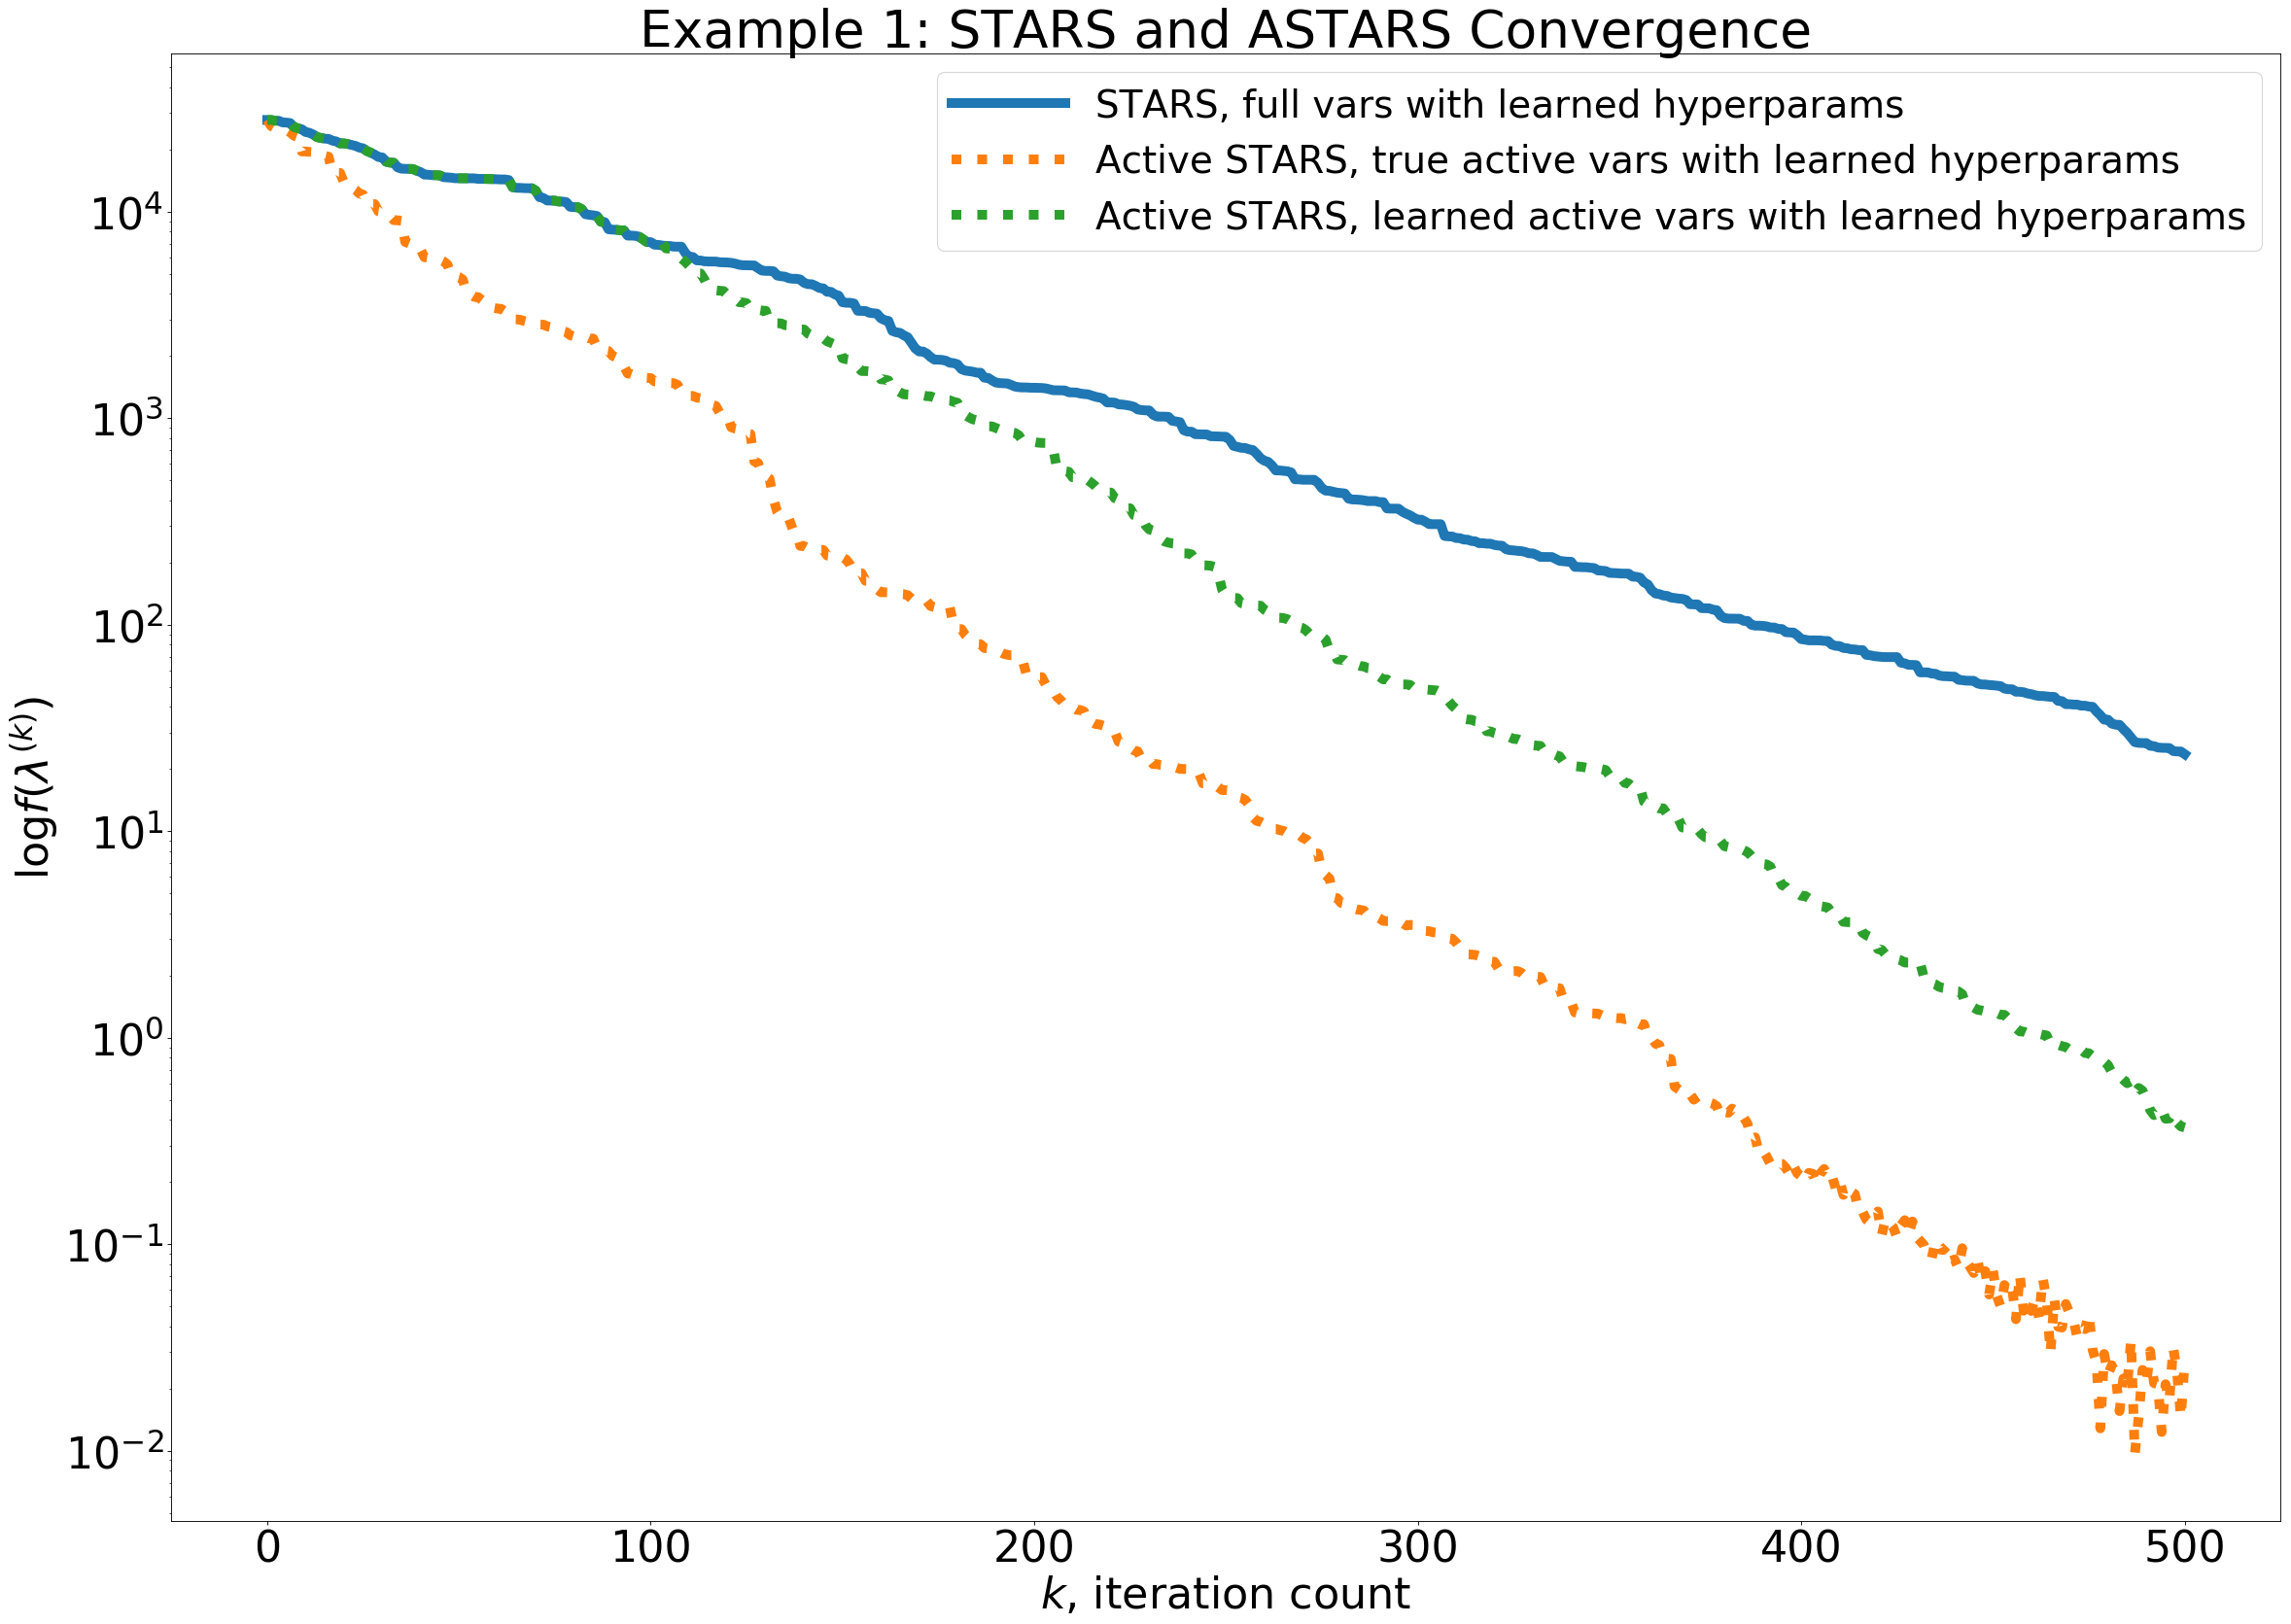
\includegraphics[scale=.14]{ex_1_pic_2} 

\textbf{Figure 1:} We present a semi-log plot showing the convergence of 500 iterations of STARS in full variables, 500 iterations of Active STARS with the exact or \textit{true} active variables, and STARS for 100 iterations followed by 400 iterations of Active STARS trained on the samples from 100 iterations of STARS.

\vspace{.5cm}

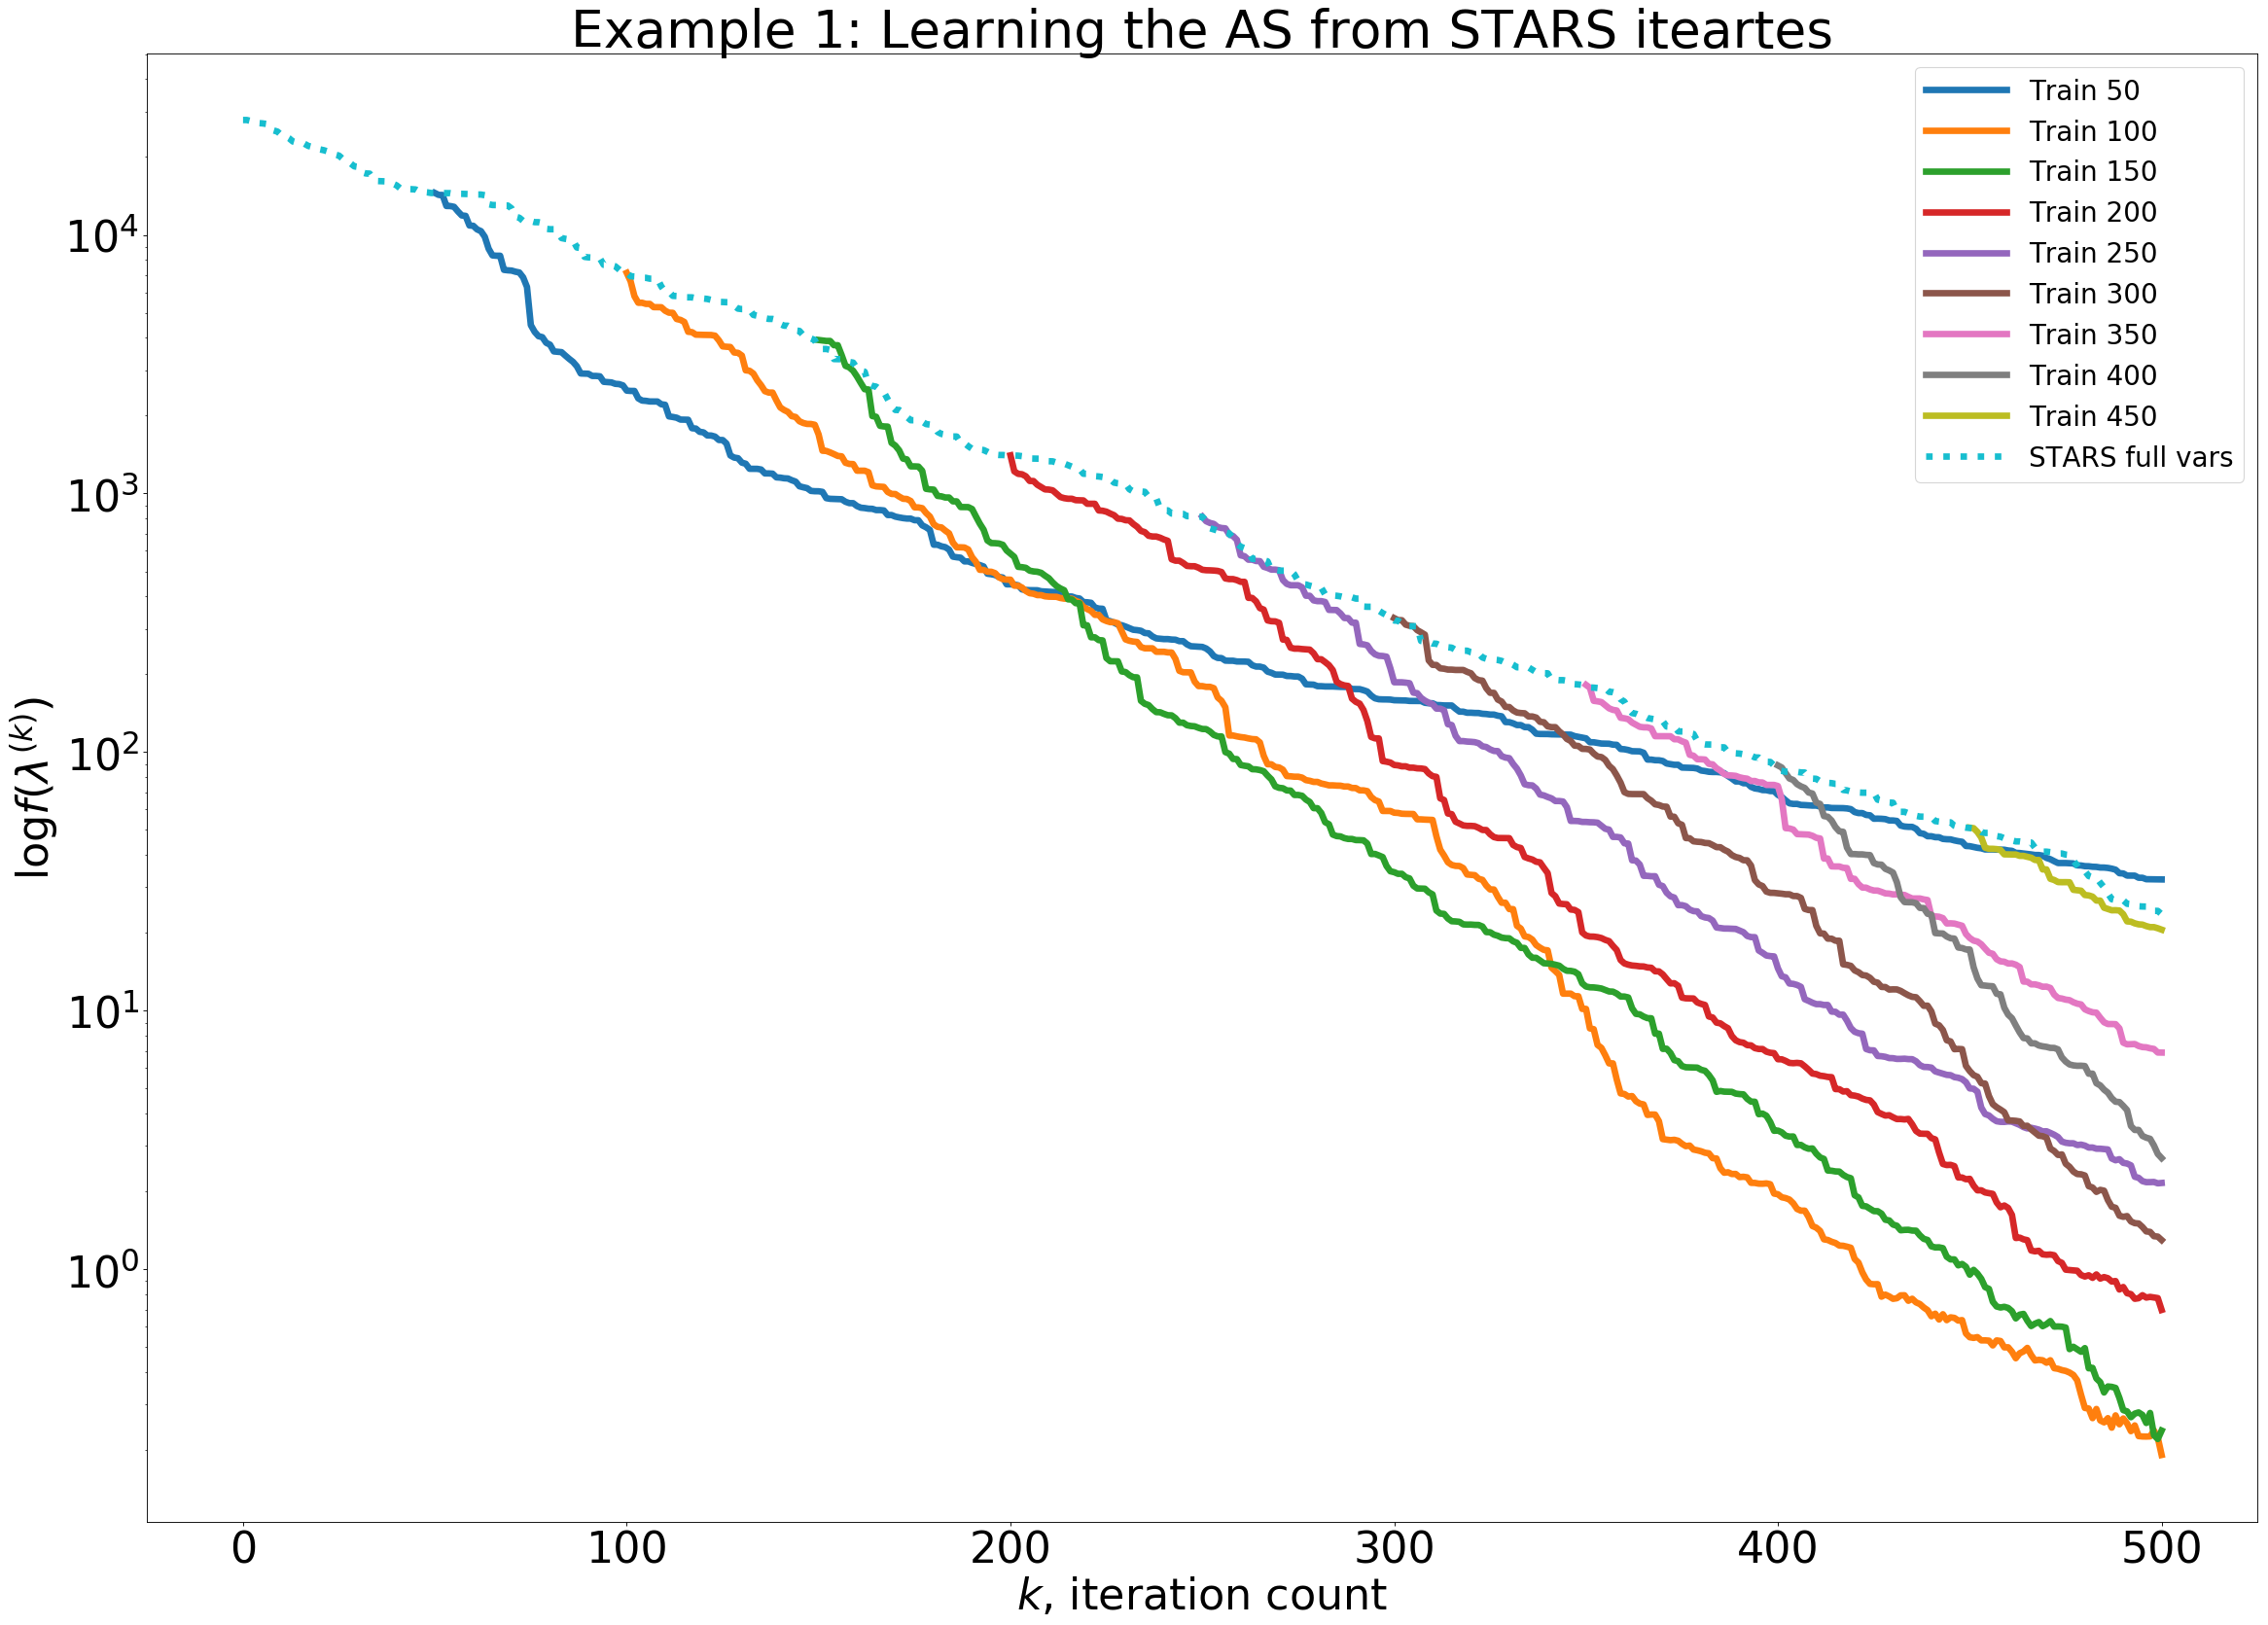
\includegraphics[scale=.14]{ex_1_pic_1}

\textbf{Figure 2:} We present a semi-log plot showing the convergence of STARS followed by Active STARS where Active STARS begins after $50,100,150,\ldots,$ and $450$ iterations of STARS. Here, the active variables have been learned from however many STARS iterates occur before Active STARS begins, along with STARS in full variables for comparison.

\end{center}

\noindent \textbf{Example 2.} \textit{Let} $f: \R^{11} \to  \R,$  

$$f(\lambda; \xi)=\sum_{i=0}^{10} 2^{(-1)^i i}\lambda_i^2+\epsilon(\xi), \quad \epsilon(\xi) \sim U[-k,k], \quad k=1 \times 10^{-2}.$$ \textit{We see $P=11$ and $D=1$. Note that the minimum of $f$ is given by $0 \in \Lambda$. Here, as $i$ increases, terms in $f$ become either more important or less important, depending on whether $i$ is even or odd. Also note that $f$ possesses additive noise with variance $\sigma^2=k^2/6.$ Here, we have 6 active variables (i.e., $j=6$) and 5 inactive variables.  We take an initial iterate $\lambda^{(0)}=(u,u,\ldots,u)$, $u \sim U[0,1]$. First, we obtain $\hat{\sigma}^2 \approx 0.02$ and $L_1^{prior} \approx 1786.5$. We note that here we have overestimated the noise by three orders of magnitude but have estimated $L_1$ to within its true order of magnitude, as here we have $\sigma^2=k^2/6\approx 1.67\times10^{-5}$ and $L_1=2\cdot 2^{10}=2048.$ Using these learned hyperparameters, we performed STARS in full variables and 2 variants of Active STARS. The first variant is performing Active STARS using the exact active variables, which in this case equal the standard basis elements in $\R^{11}$ with even indexes. The second, more realistic variant is performing Active STARS using active variables learned from the first 200 iterations of STARS. We first show convergence plots for the three approaches.  We then show convergence plots for Active STARS performed after a certain number of STARS iterations, beginning with 50 and ranging to 450, including the convergence of Active STARS trained on 200 iterations. }



\begin{center}


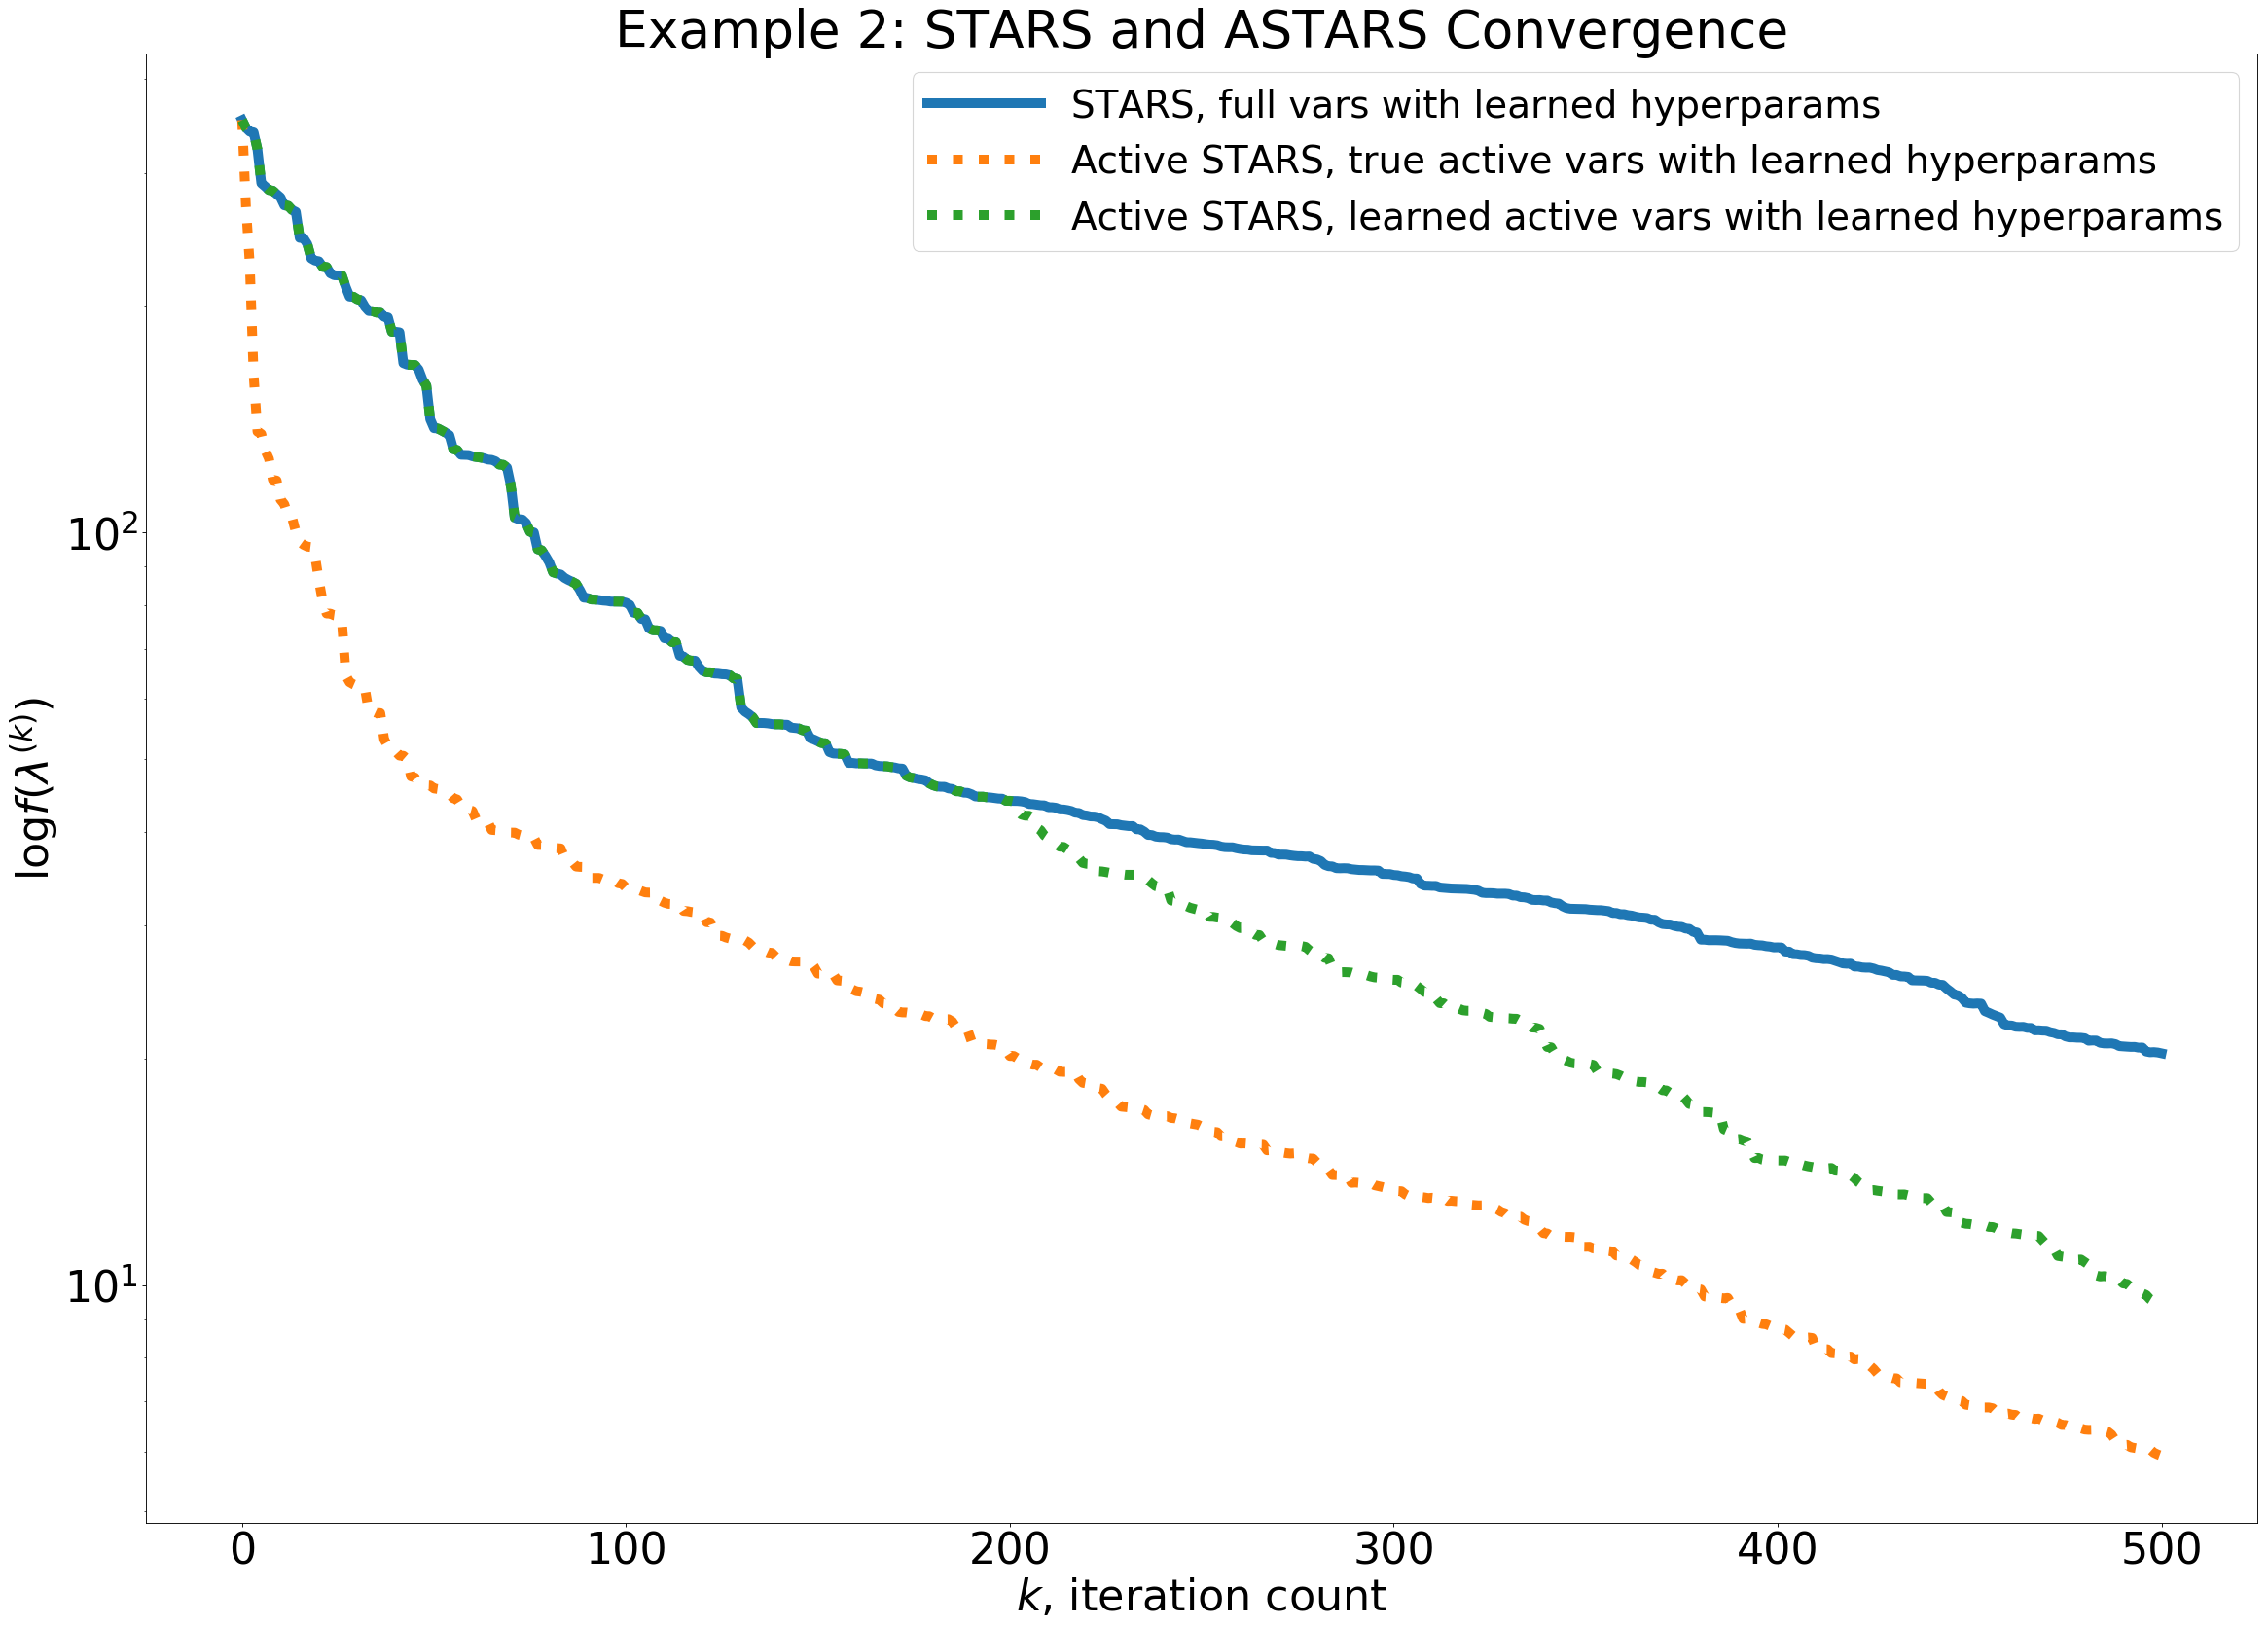
\includegraphics[scale=.14]{ex_2_pic_2} 

\textbf{Figure 3:} We present a semi-log plot showing the convergence of 500 iterations of STARS in full variables, 500 iterations of Active STARS with the exact or \textit{true} active variables, and STARS for 200 iterations followed by 300 iterations of Active STARS trained on the samples from 200 iterations of STARS.

\vspace{.5cm}

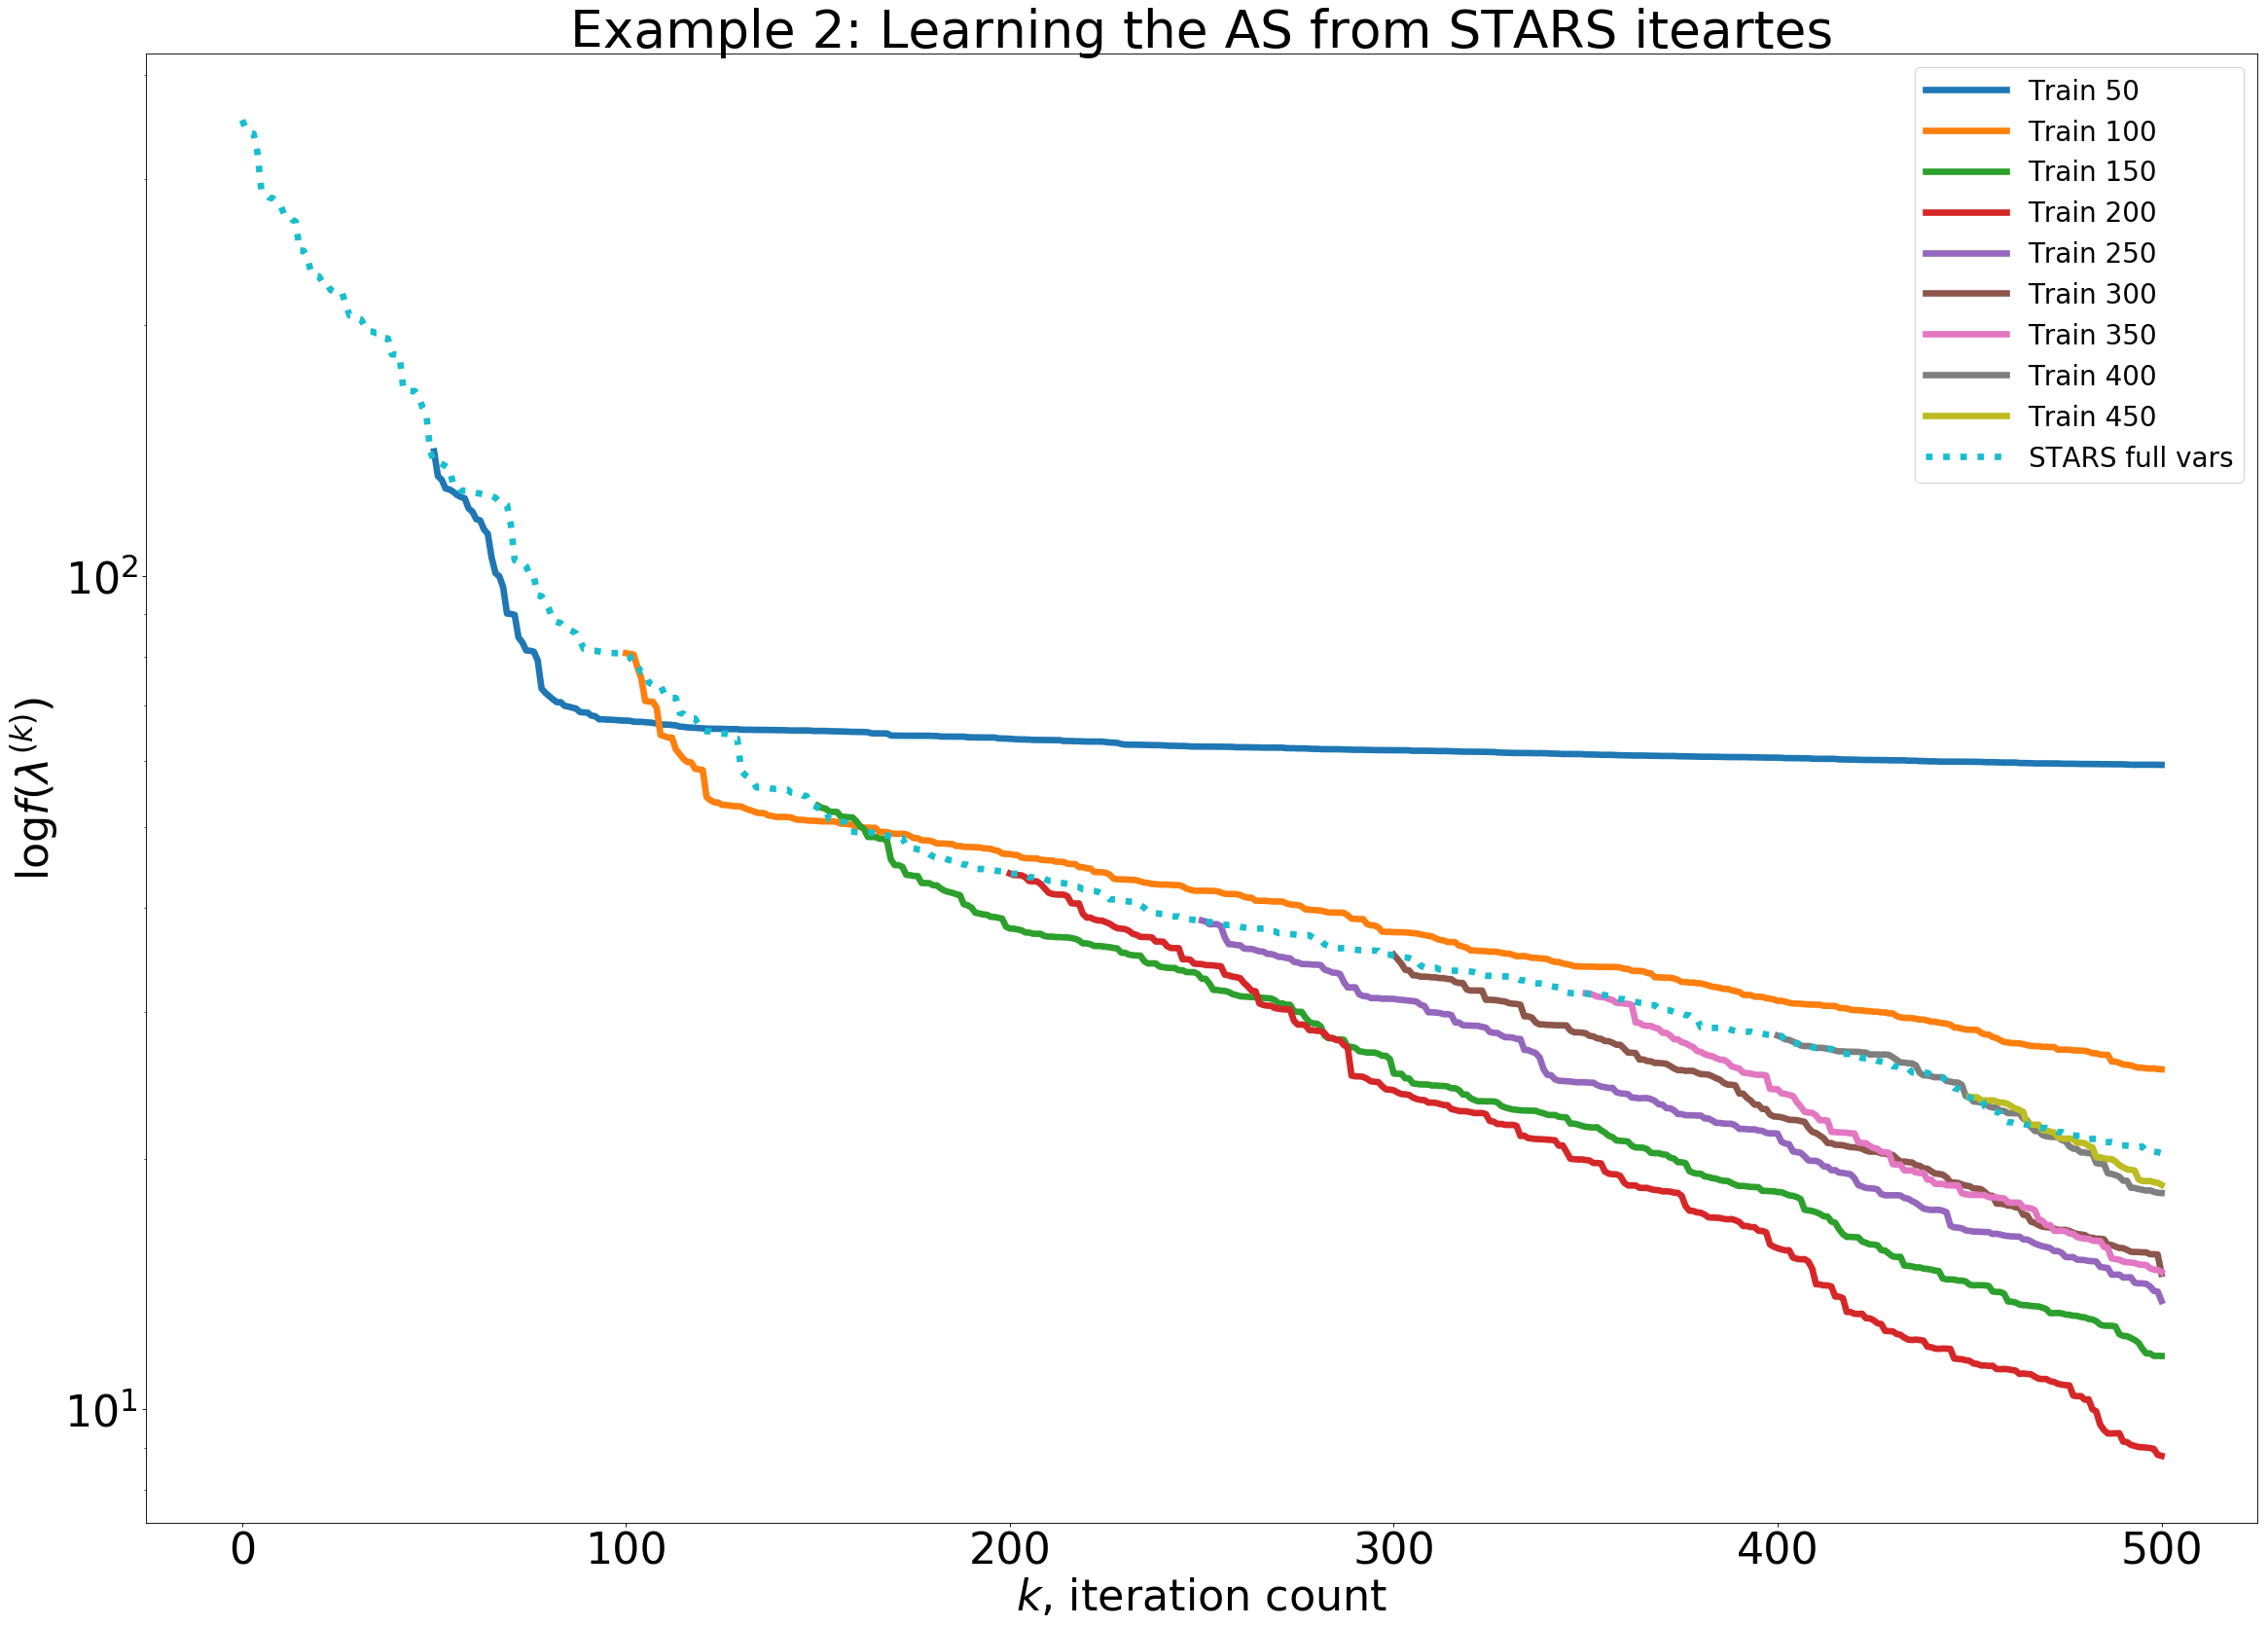
\includegraphics[scale=.14]{ex_2_pic_1}

\textbf{Figure 4:} We present a semi-log plot showing the convergence of STARS followed by Active STARS where Active STARS begins after $50,100,150,\ldots,$ and $450$ iterations of STARS. Here, the active variables have been learned from however many STARS iterates occur before Active STARS begins, along with STARS in full variables for comparison.

\end{center}



In both examples, we see the computational benefit in stepping in the active subspace instead of in the full variables. Recall that the hyperparameters in STARS are dimension-dependent, so anytime an active subspace resolves $f$ well -- which occurred in the above examples by obvious design -- we expect Active STARS in the exact active variables to converge more quickly than STARS in full variables.  

We observe that Active STARS using learned active directions may actually fail to converge at all if too few training samples are used. This is displayed clearly in Figure 4, where we see that Active STARS trained from only 50 STARS evaluations will fail to converge. However, in Figure 2, we see that with 50 training iterations, we end up with convergence similar to, or slightly worse than, STARS in full variables.






\subsection{Software Dissemination}

Software used to produce results in this paper are publicly available on \texttt{https://github.com/jordanrhall/personalresearch}. Some of the algorithms used here and other algorithms that are of interest are within open-source packages available online including those of Constantine et al
\texttt{http://activesubspaces.org}.


\section{Conclusion and Discussion} \label{s:Conc}

%In the following, we leave the reader with concluding remarks and discussion. The preceding Methods section
We presented combinations and modifications made to well-documented algorithms including STARS \cite{CW}, Monte Carlo AS learning \cite{ConstantineMC}, noise variance learning \cite{MW}, and Lipschitz constant learning \cite{Calliess} to produce the fully-automated Active STARS algorithm. In addition, we presented several model  problems that were used for testing Active STARS.

We observe  %in our Results 
that performing Active STARS can provide computational savings since its convergence outpaces STARS convergence on average. We note that at times, either algorithm may take a very \textit{lucky} step in $\Lambda$, causing quick convergence. We also observe that it is possible to learn the active subspace of the functions considered using recycled iterates from STARS, which greatly reduces the usual computational expense of an AS computation.

Of course, there is never any guarantee that the maps $f$ considered in this paper permit dimension reduction via AS. This could be the case for many reasons, including (nearly) equal importance of modeled parameters, a $\nabla f$ that is not poorly approximated by surrogates, %possible to approximate via surrogates, 
or a noise level on the same (or greater) order of magnitude as the outputs of $f$. Regardless, in the case that no active subspace is clearly defined, recall that Active STARS will simply reduce back to STARS in full variables. STARS in full variables may struggle to converge or fail to converge if $f$ possesses the behaviors described above.

Anytime the signal-to-noise ratio approaches 1, we expect failure of all methods presented. The assumptions made during the introduction forbid noise of this order, and with good reason: anytime the noise is on the order of function evaluations, it becomes difficult (and eventually impossible) to distinguish the true signal from the effects of noise. Filtering methods must be used in this scenario, which is beyond the scope of this paper. %not a topic of this paper.

%%%%%%%%%%%%%% References %%%%%%%%%%%%%%%%%%%%%%%%%
\begin{thebibliography}{65}


\bibitem{Calliess} Jan-Peter Calliess. ``Lipschitz optimisation for Lipschitz interpolation." In 2017 American Control Conference (ACC 2017), Seattle, WA, USA, May 2017.

\bibitem{CW} Chen and Wild. ``Randomized Derivative-Free Optimization of Noisy Convex Functions." Funded by the Department of Energy. 2015.

\bibitem{Constantine2015} Constantine, Paul G. ``Active Subspaces: Emerging Ideas for Dimension Reduction in Parameter Studies." SIAM, 2015.

\bibitem{ConstantineMC} Constantine, Eftekhari, Wakin. ``Computing Active Subspaces Efficiently with Gradient Sketching." Conference paper, 2015 IEEE 6th International Workshop on Computational Advances in Multi-Sensor Adaptive Processing (CAMSAP).


\bibitem{lea2000} Lea, Daniel J. and Allen, Myles R. and Haine, Thomas W. N. ``Sensitivity analysis of the climate of a chaotic system." Tellus A, Volume 52, No. 5, pp. 523-532. 2000.

\bibitem{MW} J. More and S. Wild. ``Estimating Computational Noise." SIAM J. Scientific Computing, 33(3):1292-1314, 2011. DOI: 10.1137/100786125. Funded by the Department of Energy. 2015.


\bibitem{Qiqi2014} Qiqi Wang and Rui Hu and Patrick Blonigan. ``Least Squares Shadowing sensitivity analysis of chaotic limit cycle oscillations." Journal of Computational Physics, Volume 267, pp. 210-224. 2014.

\bibitem{Russi} Russi, Trent M. ``Uncertainty Quantification with Experimental Data and Complex System Models." Dissertation, University of California Berkeley. 2010.

\bibitem{Smith}  Smith, Ralph.``Uncertainty Quantification: Theory, Implementation, and Applications.” SIAM, 2013.




\end{thebibliography}















\end{document}
